
\documentclass[10pt]{ieeeconf}

\usepackage[scheme=plain,fontset=none]{ctex}

\setmainfont{texgyretermes}[Extension=.otf,
  UprightFont=*-regular, BoldFont=*-bold,
  ItalicFont=*-italic, BoldItalicFont=*-bolditalic]
\setsansfont{texgyreheros}[Extension=.otf,
  UprightFont=*-regular, BoldFont=*-bold,
  ItalicFont=*-italic, BoldItalicFont=*-bolditalic]
\setmonofont{texgyrecursor}[Extension=.otf,
  UprightFont=*-regular, BoldFont=*-bold,
  ItalicFont=*-italic, BoldItalicFont=*-bolditalic]

\setCJKmainfont{SourceHanSerifCN-Light.otf}[Path=fonts/,
  BoldFont=SourceHanSerifCN-Bold.otf, Scale=0.98]
\setCJKsansfont{SourceHanSerifCN-Light.otf}[Path=fonts/,
  BoldFont=SourceHanSerifCN-Bold.otf, Scale=0.98]

\linespread{1.05}


\usepackage{amsmath,amssymb}
\usepackage{unicode-math}
\setmathfont{texgyretermes-math.otf}
\providecommand{\bm}[1]{\boldsymbol{#1}}

\usepackage{siunitx}
\robustify\bfseries
\usepackage{booktabs}
\usepackage{float}
\usepackage{array}


\usepackage{etoolbox}
\makeatletter
\patchcmd{\@makecaption}
  {\bgroup\par\@IEEEtabletopskipstrut}
  {\bgroup\par\centering\@IEEEtabletopskipstrut}
  {}{\ClassWarningNoLine{ieeeconf}{Table caption centering patch failed}}
\patchcmd{\ieeeconf@printoneaffiliation}
  {\texttt}{\textrm}
  {}{\ClassWarningNoLine{ieeeconf}{Email font patch failed}}
\makeatother
\graphicspath{{./}{figures/}}
\usepackage[capitalize,nameinlink]{cleveref}

\crefname{equation}{式}{式}
\Crefname{equation}{公式}{公式}
\crefname{section}{节}{节}
\Crefname{section}{节}{节}
\crefname{subsection}{节}{节}
\Crefname{subsection}{节}{节}
\crefname{figure}{图}{图}
\Crefname{figure}{图}{图}
\crefname{table}{表}{表}
\Crefname{table}{表}{表}
\crefname{appendix}{附录}{附录}
\Crefname{appendix}{附录}{附录}
\crefformat{section}{第#2#1#3~节}
\crefformat{subsection}{第#2#1#3~节}

\renewcommand{\abstractname}{摘要}
\renewcommand{\IEEEkeywordsname}{关键词}
\renewcommand{\refname}{参考文献}
\renewcommand{\figurename}{图}
\renewcommand{\tablename}{表}
\renewcommand{\appendixname}{附录}

\makeatletter
\ifieeeconf@doubleanonymous\else
  \renewenvironment{acknowledgments}{\section*{致谢}}{}
\fi
\makeatother


\newif\ifCNaFourPaper
\CNaFourPaperfalse
\ifCNaFourPaper
  \setlength{\paperwidth}{210mm}
  \setlength{\paperheight}{297mm}
  \addtolength{\textheight}{17.6mm}
  \addtolength{\oddsidemargin}{-2.95mm}
  \addtolength{\evensidemargin}{-2.95mm}
\fi

\newcommand{\RR}{\mathbb{R}}


\title{\bfseries 基于光电容积脉搏波的无袖带血压估计综述}

\addauthor{唐帅龙}{1}

\addaffiliation{1}{深圳大学， }
\addemail{1}{2410267023@mails.szu.edu.cn}

\begin{document}

\maketitle

% 摘要与关键词

\begin{abstract}
光电容积脉搏波（photoplethysmography, PPG）可由腕表、指环等设备低成本获取，是无袖带血压估计最常用的信号源；PPG与血压存在统计关联，估计精度取决于表征形式、监督标签与验证协议是否匹配。本文以如何由 PPG 估计血压为主线：说明 PPG 的生理来源及其与血压的关联，再按手工特征与传统回归、端到端深度网络、预训练并微调三条路线，比较各类方法在表征、监督与部署代价上的取舍，并讨论个体化校准与多模态融合；随后整理常用数据集与临床评价标准，并讨论数据划分与校准隔离对结论可比性的影响。目前，血压估计的方法重心已由特征设计转向表征学习与个体校准，进一步提升的瓶颈则在于数据质量与评测协议；人群差异、校准负担与标签稀缺仍是走向实用的主要障碍。
\end{abstract}

\vspace{0.45\baselineskip}


% ============================================================================
% 引言
\section{引言}
\label{sec:intro}

高血压是最常见的慢性心血管疾病风险因素，长期控制不佳会显著增加脑卒中与心力衰竭风险\cite{kario2024who}。但袖带式设备依赖间歇充气，难以满足长时程监测需求，因此连续、无感的血压监测具有重大的临床价值。

光电容积脉搏波通过光学方式观测皮下微血管的血容量变化，可集成于智能手表、指环与耳戴设备，具备低成本、低功耗、易佩戴的优势。其波形形态与动脉顺应性、外周阻力、脉搏波传导时间等因素相关，因而与收缩压、舒张压存在统计关联\cite{charlton2022wearable,tang2026sifpbpnet}；但这种关联受血管张力、体温、体位与个体差异调制，并不构成确定的物理方程，估计问题最终归结为映射学习，精度取决于表征形式、监督标签与验证协议三者的匹配。本文以如何由 PPG 估计血压为主线，围绕表征、监督与验证三个环节进行综述。

\noindent 本文的主要内容可概括为：梳理 PPG 的生理学基础与信号特征，说明其与血压的统计关联及局限；按手工特征与传统回归、端到端深度网络、预训练并微调三条路线，比较各类方法在表征、监督与部署代价上的取舍，并讨论个体化校准与多模态融合；汇总常用数据集与评价标准，分析验证协议对结论可靠性的影响，并分析人群差异、校准与标签稀缺等问题。

本文组织结构如下：\cref{sec:physio}介绍生理基础与波形特征；\cref{sec:techniques}比较三类估计方法；\cref{sec:datasets}介绍数据集与评价标准；\cref{sec:challenges}总结挑战与未来方向；\cref{sec:conclusion}给出结论。

% ============================================================================
% 生理学基础与信号特征
\section{生理学基础与信号特征}
\label{sec:physio}

\subsection{PPG原理与测量条件}
\label{sec:ppg_principle}

PPG 信号是由发光二极管照射皮肤，再由传感器接收透射或反射光强得到的信号。心脏射血期动脉血容量增加，血红蛋白对光的吸收增强，接收光强随之下降，形成上升支；舒张期血液回流、血容量减少，光强回升，形成下降支\cite{allen2007photoplethysmography}。采集到的信号可分解为随心跳搏动的交流（AC）分量与缓慢漂移的直流（DC）分量：前者反映搏动性灌注，后者由皮肤、静脉血与佩戴压力共同决定。PPG本质上是血容量脉搏的光学观测，而非动脉压力波形本身\cite{reisner2008utility}。

另外，测量条件会系统性地影响波形。波长决定探测深度，绿光主要反映浅层毛细血管的容积变化，近红外光可穿至更深的皮下小动脉；测量部位决定光路形式，指端多为透射式，腕部与耳部则为反射式；接触压力过大将压迫血管、过小则光耦合不足，两者都会压低 AC 幅度并使形态失真\cite{allen2007photoplethysmography}。这些差异意味着不同设备、不同佩戴位置采集的波形并非同一分布，是\cref{sec:challenges}中跨设备泛化问题的来源之一。

\subsection{波形形态与特征点}
\label{sec:ppg_morphology}

如\cref{fig:ppg_wave}所示，一个心动周期的波形通常呈双峰形态：主峰之后，来自外周的反射波叠加形成次峰，两峰之间的凹陷即重搏切迹。当动脉硬化使反射波提前到达时，次峰向主峰靠拢乃至融合、切迹消失。

一个心动周期的形态学特征点包括：收缩期起点、收缩期主峰、重搏切迹与舒张期峰值。实际中形态学特征提取的时候多借助一阶、二阶导数辅助定位，以提高噪声下的稳定性\cite{cisnal2024robust}。由这些特征点点可进一步导出上升时间、主峰幅度、脉搏波面积与分支宽度等参数\cite{millasseau2006contour,cisnal2024robust}。

手工特征大致可分为三类：时域特征（时间、幅度及其比值、分段面积）、频域特征（功率谱分布与谐波结构）、导数域特征（一阶导数反映上升速率，二阶导数放大重搏切迹等细微结构）\cite{allen2007photoplethysmography,cisnal2024robust}。上述特征以特征点定位稳定准确为前提，因此特征点检测在噪声下的稳定性，往往比特征本身更能决定最终精度。

\begin{figure}[t]
\centering
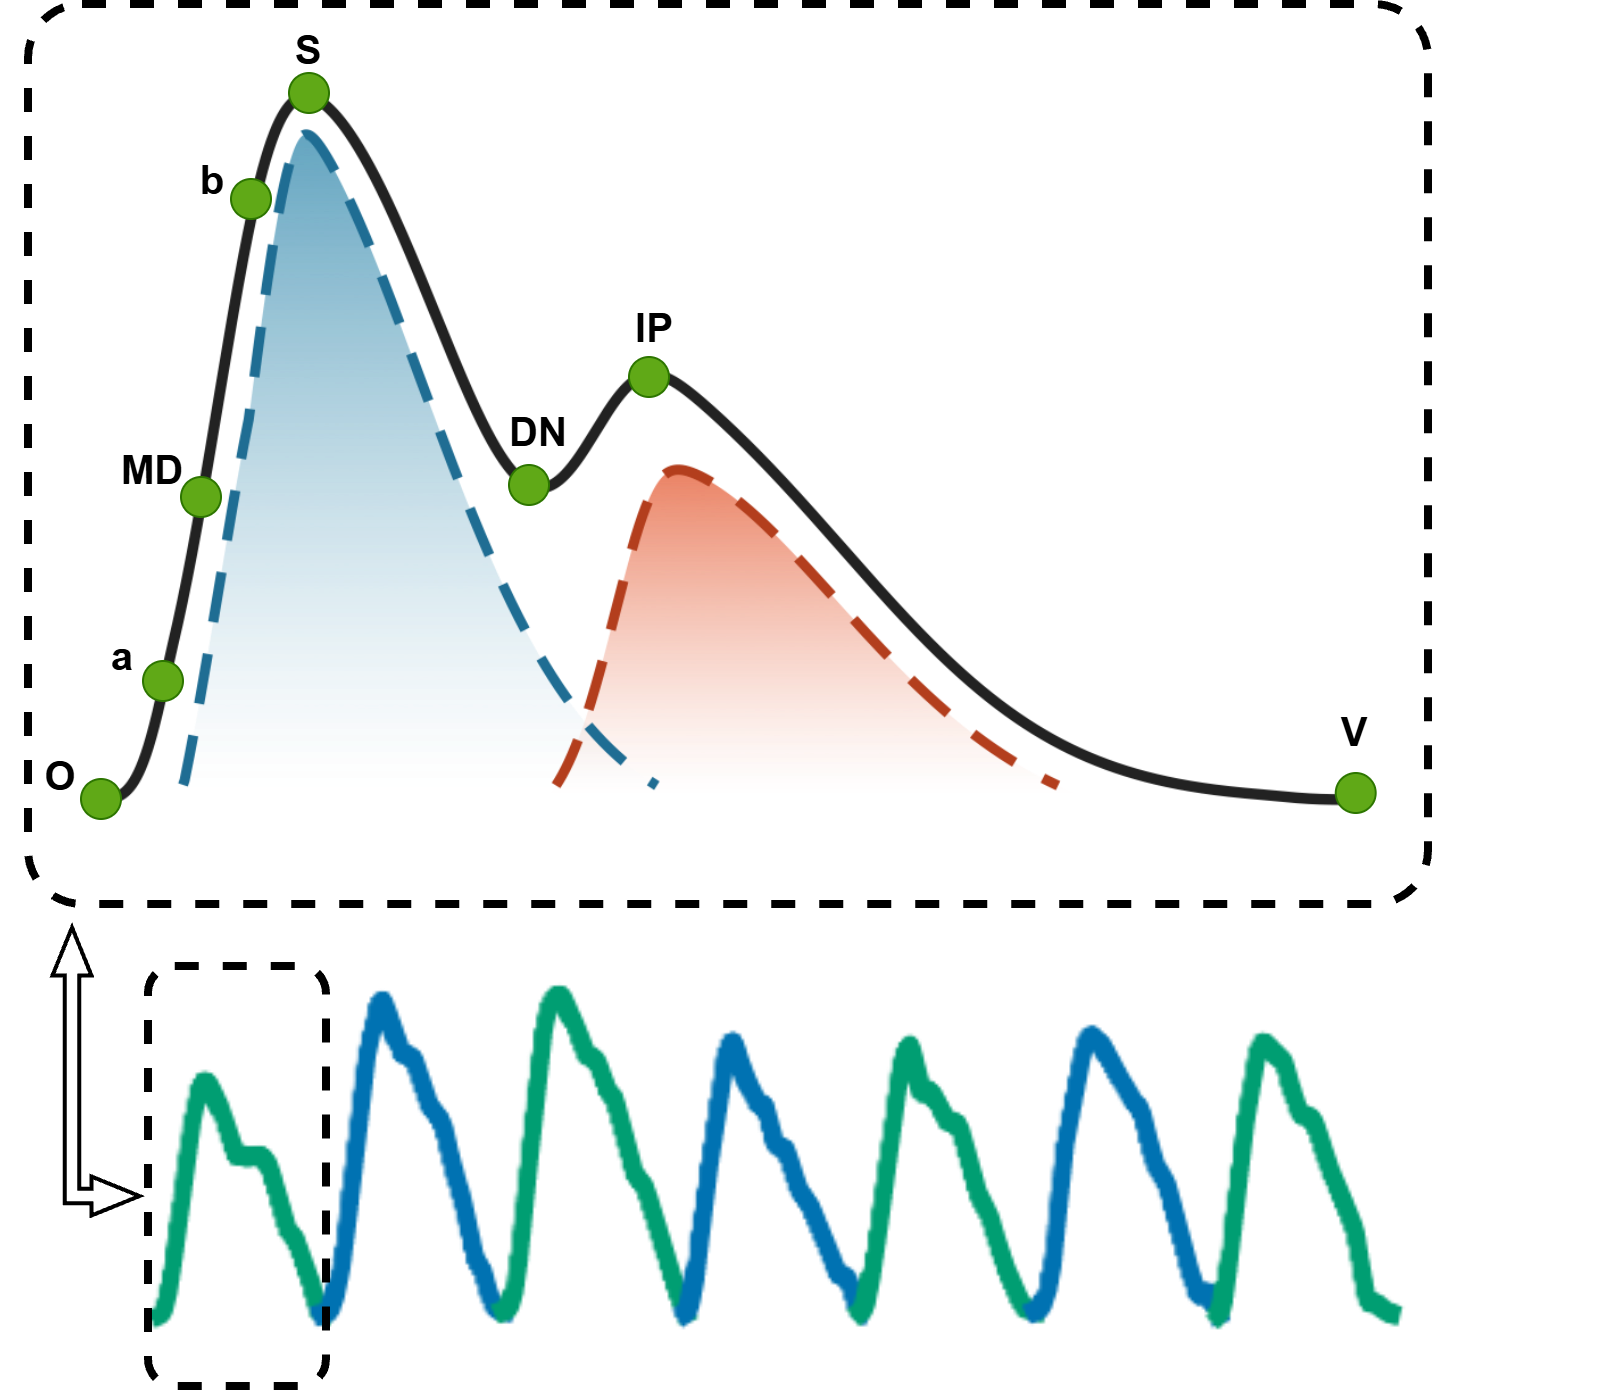
\includegraphics[width=\columnwidth]{3_生理学基础及信号特征/ppg_feat.drawio.png}
\caption{PPG 波形与基准点。单周期波形可视为前向波（蓝）与外周反射波（橙）叠加的结果，黑色曲线为单周期波形；特征点中O为收缩期起点、S 为主峰、DN 为重搏切迹、IP 为由反射波形成的次峰。}
\label{fig:ppg_wave}
\end{figure}

\subsection{与血压的生理关联}
\label{sec:ppg_bp}

PPG 信号本身携带心血管信息，这些信息隐含在波形之中，并可由上述特征反映出来。具体到血压任务，其物理基础在于波的传播：脉搏波沿动脉树传至外周再反射回来，波速由管壁弹性决定，血压升高时管壁张力增大、波速加快，反射波提前返回并在收缩期与前向波叠加，使切迹上移。

一些 PPG 形态学参数具有明确的生理学含义：次峰与主峰的幅度之比即反射指数（reflection index, RI），反映外周血管的反射强度，随年龄与血管状态系统性变化；上升时间与上升支斜率反映心室射血速度与动脉顺应性；主峰幅度、曲线下面积与 AC/DC 灌注指数则与每搏输出量和外周灌注水平相关\cite{millasseau2006contour,allen2007photoplethysmography,elgendi2019use}。时间维度上则是脉搏波传导时间（pulse transit time, PTT）：血压升高时波速加快、PTT 缩短，二者呈负相关，早期研究据此在间歇校准下连续估计收缩压\cite{chen2000continuous,poon2005cuffless}。只用单路 PPG 时，可用两峰间期 $\Delta T$（主峰至次峰的时间）作为波速的替代量——它对应脉搏波在主动脉与外周反射点之间的往返行程，与波速成反比，大动脉硬化时随之缩短\cite{millasseau2006contour}。这些参数与收缩压、舒张压确实存在统计相关，但相关强度受血管张力、体温、体位、呼吸与交感神经活动的调制，个体间差异显著，同一个体在不同时段的映射也会漂移\cite{lin2020investigating,yang2020estimation}。

综上，这些参数的生理含义虽然明确，但其与血压的相关强度随生理状态与个体而变，因此二者之间并不存在确定性的物理方程，只存在统计关系。基于此，血压估计被归结为一个映射学习问题：由一段 PPG 波形（或其派生特征）回归收缩压与舒张压，必要时还需要借助血压基线完成个体校准；用哪些特征也不能靠人工设计一劳永逸，而要由模型从数据中自行学习。这一转变构成\cref{sec:techniques}的主线。



% ============================================================================
% 技术发展

\section{血压估计方法}
\label{sec:techniques}

\subsection{方法框架与演进}
\label{sec:evolution}

PPG估计血压模型需要考虑四个问题：输入用什么表征、采用什么模型、监督信号从哪里来、是否使用受试者的个性化数据。可以把现有工作划为三条路线，\cref{fig:routes}(a) 中使用不同的颜色表示不同的路线：手工特征配合浅层回归的传统机器学习路线（蓝）、端到端深度学习路线（紫），以及先大规模预训练再微调的路线（橙）。三条路线都可以实现血压估计，差别主要在监督来源与部署成本：传统路线依赖于手动特征与血压标签；端到端路线通过深度学习网络学习表征，但需要更多带标签数据；预训练路线先在大量的无标注PPG上学习通用表征，再用少量标签完成下游微调。

\begin{figure*}[t]
\centering
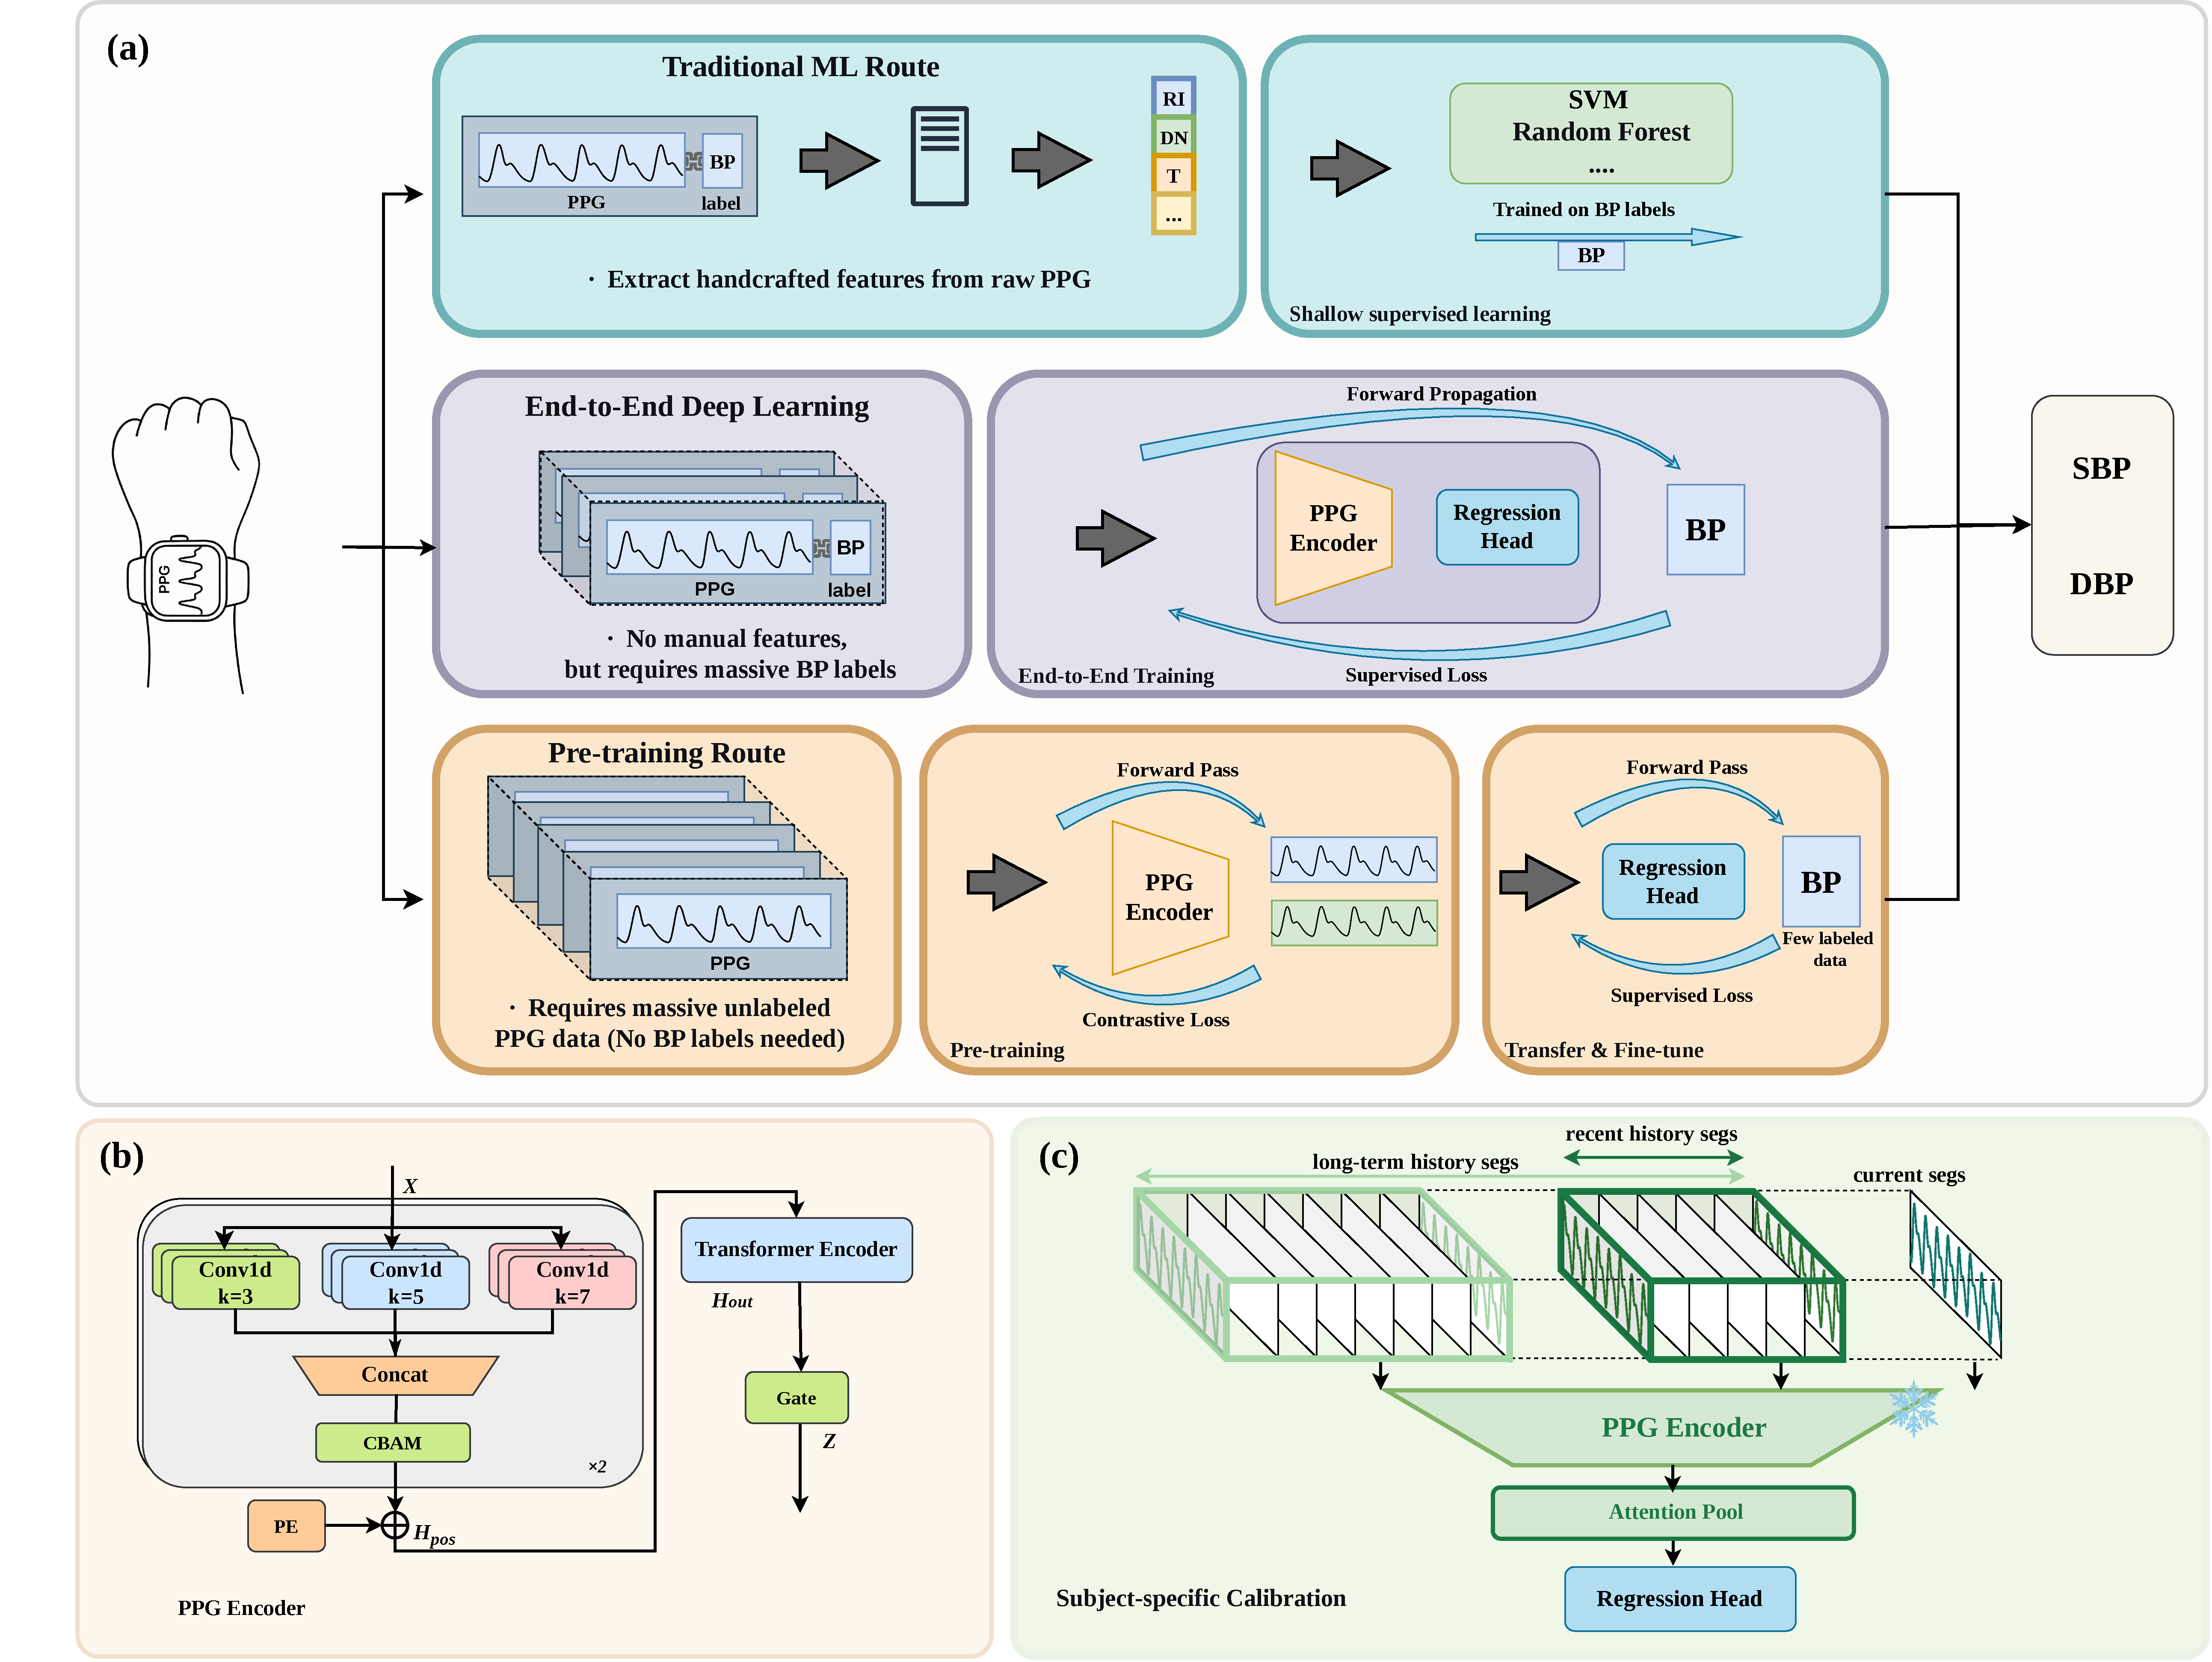
\includegraphics[width=\textwidth]{4_血压估计方法/figs/三路线图.drawio.pdf}
\caption{由 PPG 估计血压的方法框架。(a) 三条技术路线：传统机器学习（蓝）、端到端深度网络（紫）与预训练—微调（橙），三者在输入表征、监督信号与校准数据上各有取舍；(b) PPG编码器（SIFPBPNet）：原始波形及其一、二阶导数构成三通道输入，经多尺度一维卷积、CBAM 注意力、位置编码与 Transformer 编码器得到片段表征；(c) 个体化校准：长期与近期历史片段经冻结的编码器与注意力池化聚合成稳态表征，与当前片段融合后回归个体血压。}
\label{fig:routes}
\end{figure*}

手工特征路线以\cref{sec:physio}讨论的形态、频域与导数域特征为输入，配合支持向量机、随机森林或多线性回归估计血压\cite{haddad2022continuous,cisnal2024robust}。其特征有明确的生理含义，模型可解释、训练代价低，在连续监测中应用较广；但特征依赖先验，对运动伪影与佩戴松紧敏感，换数据集常需重做特征筛选，跨库迁移时性能衰减明显。这一局限把研究推向端到端学习。

三条路线共同的难点是个体差异：同一段波形在不同受试者身上可能对应不同血压水平，人群模型倾向于向均值回归。\cref{fig:routes}(c) 所示的个体化校准则为缓解这一问题而引入，后文\cref{sec:calib}展开。

\subsection{端到端深度网络与 PPG 编码器}
\label{sec:deep}

端到端路线让网络直接从原始波形或时频表示回归血压。CNN是较早的用于回归血压的深度学习模型\cite{liu2019cuffless}，此后循环网络与Transformer相继引入：卷积擅长局部形态，循环结构建模逐拍依赖，注意力机制便于融合多通道信息，三者常被组合使用。在这一路线中编码器的设计十分关键，\cref{fig:routes}(b) 为SIPFBP的PPG编码器结构：输入为原始 PPG 及其一阶、二阶导数构成的三通道信号；三路并行的一维卷积分别取 $k=3,5,7$ 的感受野，提取不同时间尺度的局部形态；拼接后经 CBAM 的通道与空间注意力抑制噪声、突出与血压相关的区域；再叠加位置编码保留片段的绝对时序，送入Transformer实现的长程表征提取；最后经全局池化与门控得到片段表征。

\cref{fig:routes}(b)的结构展现了目前编码器的共同取向：多尺度卷积负责局部形态，注意力负责特征选择与时序建模，表征由数据驱动。代价是需要大量有标签的样本，且中间表征难以对应到具体的生理解释，可解释性弱。一个合适的编码器既可以使用端到端的方式训练，也可以用无监督预训练的方式进行训练。

\subsection{大规模预训练}
\label{sec:pretrain}

预训练路线对应\cref{fig:routes}(a) 的橙色分支：先在海量无标注片段上预训练编码器，再用少量标注数据微调下游回归头。掩码重建与对比学习为此提供了成熟范式\cite{he2022mae,chen2020simclr}；PaPaGei 与 AnyPPG 将这一范式带到 PPG，借助大规模记录学习通用表征\cite{pillai2025papagei,nie2025anyppg}。近期的改进集中在掩码粒度与先验引入：HiMAE 用分层掩码同时保留粗、细两种时间尺度\cite{lee2026himae}，另有工作按小波分解的多尺度结构组织掩码单元、以外周参考信号引导跨模态重建\cite{thukral2026wavelet,zhou2026physiology}。另一个方向是让掩码单元与生理节律对齐：以完整心动周期作为掩码的基本单元，并借助受试者的纵向历史片段提供个体上下文，可避免跨心搏掩码造成的语义混杂。

预训练的价值在于缓解血压标签稀缺：无标注 PPG 易于大规模采集，而同步袖带标签昂贵且稀疏。其局限是预训练目标与血压回归之间存在语义差距，微调阶段仍需一定数量的标签，且不同预训练语料带来的增益在跨设备场景下并不稳定。

\subsection{个体化校准与多模态融合}
\label{sec:calib}

预训练解决通用表征，个体差异仍需在部署端处理。常见做法分三档：一次袖带测量做单点校准、按时段重复校准，或用元学习与少样本微调快速适配新受试者；仅用数分钟个体数据训练混合推理模型，可把免频繁校准的可用期延长到月级\cite{mekonnen2024accurate}。

\cref{fig:routes}(c) 给出一种更系统的校准思路：不直接把当前片段映射到血压，而是先从用户的历史片段中挖掘个体稳态信息。具体而言，长期与近期的历史片段与当前片段经冻结的 PPG 编码器得到表征；历史片段的表征以注意力池化聚合为稳态表征，刻画该用户的血压基线与波动模式；稳态表征再与当前片段表征融合，经回归头输出个体化血压。SIFPBPNet 以图注意力网络聚合数量可变的历史片段，并用年龄回归、高血压判别与血压变异性检测等辅助任务预训练该路径，使稳态表征携带与血压相关的个体先验，两阶段训练中历史数据与评估数据按受试者隔离\cite{tang2026sifpbpnet}。该模块可即插即用地接入不同骨干网络，在多个骨干上带来收缩压 MAE 2.8\%--13.1\% 的相对降低。

另外就是多模态融合：在 PPG 之外引入毫米波脉搏波、心电或加速度计，补充压力波形与运动信息\cite{zheng2024bp3,mieloszyk2022comparison}。校准与融合的共同代价是部署复杂度：前者需要历史数据与隐私保护，后者需要额外传感器与同步采集。

\subsection{小结}
\label{sec:techniques_summary}

血压估计的方法的重心已从设计特征移到学习表征，再移到学表征并校准个体。\cref{fig:routes} 的三部分恰好对应此变化过程：\cref{fig:routes}(a)：路线选择决定监督来源，\cref{fig:routes}(b)：编码器设计决定表征质量，\cref{fig:routes}(c)：个体化校准决定部署后的精度保持。模型容量与预训练规模仍在快速提升，但跨数据集、跨设备的性能衰减尚未根本解决；能否在有限校准数据下保持鲁棒，仍是区分方法优劣的关键。

% ============================================================================
% 数据集与评估标准
\section{数据集与评估标准}
\label{sec:datasets}

\subsection{常用数据集}
\label{sec:dataset}

\cref{tab:datasets}汇总了由 PPG 估计血压常用的公开数据集，它们的采集场景差别明显。VitalDB 与 MIMIC-III 取自手术室与 ICU，参考血压为同步的动脉线，标签连续、时间分辨率高，但人群的血压分布偏病理，向健康人群迁移时需重新验证\cite{lee2022vitaldb,johnson2016mimic}。Aurora-BP、PPG-BP 与 VV 以袖带测量为参考，多为静息状态下的短时记录，适合片段级回归\cite{mieloszyk2022comparison,liang2018ppg,toye2023vital}；其中 Aurora-BP 同步采集 PPG、ECG 与动脉张力，并覆盖卧、坐、站等体位，是腕表场景下少见的带标签数据。总体而言，连续参考的数据集中在临床监护场景，袖带参考的数据偏静息单次测量，能够反映日常活动状态的公开数据仍然稀缺。

\begin{table}[t]
\centering
\caption{常用公开数据集及其参考血压来源}
\label{tab:datasets}
\footnotesize
\setlength{\tabcolsep}{3.5pt}
\begin{tabular}{@{}lrrrl@{}}
\toprule
数据集 & 受试者 & 时长 (h) & 采样率 (Hz) & 位置 / 标签 \\
\midrule
VitalDB & 5\,866 & 17\,355 & 500 & 指端 / ABP \\
MIMIC-III & 5\,596 & 19\,990 & 125 & 指端 / ABP \\
Aurora-BP & 1\,206 & -- & -- & 腕部 / 袖带 \\
PPG-BP & 219 & -- & 1\,000 & 指端 / 袖带 \\
VV (SkinTone) & 231 & -- & 60 & 指端 / 袖带 \\
\bottomrule
\end{tabular}
\end{table}

\subsection{评价指标}
\label{sec:metrics}

设 $\hat{y}_i$、$y_i$ 为第 $i$ 个样本的估计值与参考值，$N$ 为样本数，则平均绝对误差与均方根误差定义为
\begin{equation}
\mathrm{MAE}=\frac{1}{N}\sum_{i=1}^{N}\left|\hat{y}_{i}-y_{i}\right|,
\end{equation}
\begin{equation}
\mathrm{RMSE}=\sqrt{\frac{1}{N}\sum_{i=1}^{N}\left(\hat{y}_{i}-y_{i}\right)^{2}}.
\end{equation}
一致性分析报告误差均值（ME）、标准差（SD）与 Bland--Altman 的 95\% 一致性界限；SBP 与 DBP 应分别给出，不能只报二者的平均。

临床可接受性常借用 BHS 与 AAMI/ISO 81060-2 的判据（\cref{tab:standards}）。BHS 按误差落在 $\pm5$、$\pm10$、$\pm15$\,mmHg 内的累积百分比分 A--D 四级，SBP 与 DBP 分别评级、取较差者；AAMI/ISO 81060-2 要求 ME $\le5$\,mmHg、SD $\le8$\,mmHg，受试者不少于 85 人、每人至少 3 组与听诊参考的配对测量\cite{obrien1993bhs,aami2013standard}。两者均以听诊为参考，而PPG研究多以商用袖带电子血压计提供标签，参考值本身就有误差，需注意协议与人群构成的差异。

\begin{table}[t]
\centering
\caption{BHS 分级与 AAMI/ISO 81060-2 判据}
\label{tab:standards}
\footnotesize
\setlength{\tabcolsep}{3.5pt}
\begin{tabular}{@{}lcccc@{}}
\toprule
标准 & 等级 & $\le5$\,mmHg & $\le10$\,mmHg & $\le15$\,mmHg \\
\midrule
BHS & A & 60\% & 85\% & 95\% \\
    & B & 50\% & 75\% & 90\% \\
    & C & 40\% & 65\% & 85\% \\
    & D & $<$40\% & $<$65\% & $<$85\% \\
\midrule
AAMI/ISO & \multicolumn{4}{c}{ME $\le5$\,mmHg\quad SD $\le8$\,mmHg} \\
\bottomrule
\end{tabular}
\end{table}

\subsection{验证协议与可复现性}
\label{sec:protocol}

评估结论对划分方式高度敏感：片段级随机划分会让同一受试者的片段同时出现在训练与测试集，系统性高估性能，只有受试者独立划分才反映跨个体泛化；小样本常用留一受试者交叉验证，跨数据集验证则进一步检验跨设备、跨人群的迁移性。

校准协议同样影响结论：无论单点校准、按时段重复校准还是使用历史片段，校准数据都必须与测试集严格分离，否则指标会明显偏乐观。因此比较方法时应同时报告划分方式、校准数据来源与受试者数量，而不只是误差均值。

% ============================================================================
% 挑战与未来展望

\section{挑战与未来展望}
\label{sec:challenges}

\subsection{当前面临的主要挑战}
\label{sec:open_issues}

\noindent\textbf{人群差异：}血管弹性、外周阻力、皮肤色素与佩戴位置因人而异，同一 PPG 波形在不同人群中的血压映射并不一致；在手术、ICU 等特定人群上训练的模型，迁移到健康人群或跨设备场景时误差明显上升。

\noindent\textbf{个性化校准：}腕部 PPG 与上臂袖带血压的关系受外周血管与姿势影响，通常需要基线校准；单点校准难以覆盖昼夜与状态变化，频繁校准又影响可穿戴体验，如何利用个人历史数据中的稳态信息、以尽量少的校准跟踪个体漂移，尚无统一方案。

\noindent\textbf{标签稀缺：}可靠的血压标签依赖袖带或动脉线，采集成本高，公开数据或来自手术与 ICU、或为静息短时记录，腕部带标签数据尤其稀少；标签还含测量误差与时间不同步，而无标签 PPG 虽易获取，却难以直接用于监督学习。

\subsection{未来研究方向}
\label{sec:future}

针对上述挑战，可以从三个方向展开研究。其一，跨人群泛化：按年龄、肤色、体位等分层评测，结合域自适应与个性化微调，降低对特定人群的依赖。其二，低负担校准：利用个人历史片段中的稳态信息与少样本学习，在单点甚至零校准条件下完成适配。其三，标签高效学习：以自监督预训练利用海量无标签 PPG，结合弱标签与迁移学习。


% ============================================================================
% 结论

\section{结论}
\label{sec:conclusion}

本文梳理了PPG血压估计方法的生理基础、三类估计方法以及数据集与评价标准。总体来看，方法已从手工特征走向端到端表征学习，并进一步借助大规模预训练与个体化校准提升跨人群适应性；但人群差异、校准负担与标签稀缺仍是制约落地的关键。

因此，精度提升的瓶颈已由模型结构转向数据质量与评测协议：在统一的受试者级划分与校准隔离下比较方法，比继续堆叠网络容量更有价值。未来工作应围绕跨人群泛化、低负担校准与标签高效学习展开。

% ============================================================================
% 参考文献
% ============================================================================
\clearpage
\begingroup
\linespread{1.0}
\bibliographystyle{IEEEtran}
\bibliography{refs}
\endgroup

\end{document}